\chapter{X-ray Sources in Multiple Source Catalogs}
\label{chap3}

Despite the fact that imaging X-ray astronomy has had a short history compared to other sub-fields, X-ray missions have provided plenty of data and source catalogs. 
Some of those were highlighted in the previous sections. 
We set a goal of finding X-ray data that spans the longest baseline possible.
Therefore, we choose to work with the Einstein Two- Sigma Catalog (ETS), the Second Rosat All Sky Survey (2RXS), and the second release of the Chandra Source Catalog (CSC2.0). 
Comparing the catalogs, however, is not as simple as it may appear. 
This is largely due to the varying optical capabilities of each telescope.

\section{Comparing Telescope Optics}
\label{sub3_1}

Because Einstein, ROSAT, and Chandra all had different scientific goals and because they were constructed at different points in time, their telescope optics differ drastically in certain respects. 
However, they all also have components that are similar to each other. 
One main component that is the same is the mirror assembly of each. 
As could have been noted from the previous sections, all telescopes have a grazing incidence Wolter type 1 mirror assembly.
Einstein’s had a diameter of 56 cm, ROSAT had a diameter of 83.5 cm, and Chandra’s is 1.2 m.

Because of technological advances that have been made between the time Einstein and Chandra, the manufacturing of the optics plays a key role in the differences between the telescopes as well.
The surface of ROSAT's mirror was smoother, with roughness variations on micron scales, than those on Einstein. 
Chandra comes closer to achieving an ideal surface than ROSAT, so the center of the Chandra's PSF is narrower than the PSF for ROSAT. Additionally, the gas-filled IPC and PSPC detectors do not localize events as well as a CCD, so the PSF of the Einstein and ROSAT are broaden even more.

Another important comparisons can be made from each of the telescopes instruments that were used to construct the catalogs that are being considered. 
For the ETS, Einstein’s IPC focal instrument was used, ROSAT used the PSPC, and Chandra largely used ACIS-I. 
Chandra’s ACIS instrument is more detailed, more sensitive, and provides the finest spatial resolution of the three.
ROSAT has worse spatial resolution than Chandra but has the largest field of view of the three instruments.
Table 3.1 displays these properties for the instruments. 
These properties result in source position uncertainties that are very different. 
In fact, the source position uncertainties for the ETS and the 2RXS are much more substantial than those for the CSC2.0.


\begin{table}[H]
    \centering
    \begin{tabular}{cccc}
    \hline
    \hline
          &Resolution & Field of View & Effective Area (at 1 keV) \\
         \hline
        Einstein IPC    & 1'&$75' \times 75'$   & 100 cm$^2$ \\
        %
        ROSAT PSPC    &  0.25'  &  $2^{\circ}\times 2^{\circ}$ & 240cm$^2$  \\
        %
        Chandra ACIS & 0.5'' & $16.9' \times 16.9'$ & 340 cm$^2$ \\
    \hline
    \hline
    \end{tabular}
    \caption{Properties of the focal instruments on the Einstein \citep{giacconietal1979}, ROSAT \citep{Briel1996}, and Chandra \citep{Evans2020}.}
    \label{tab:my_label}
\end{table}

One major component that these surveys have in common (and the main reason why they were chosen) is the energy bands in which they are most sensitive. Einstein’s IPC operated in the 0.16 - 3.5 keV energy band, the PSPC in the 0.1 - 2.4 keV band, and  Chandra’s ACIS in the 0.3-8 keV band. 
A range where they are all sensitive (and the range which was selected to calculate flux values) is the 0.5 - 2.0 keV band. 
Thus, from the properties presented, it is clear that comparisons (handled with extreme care) can be made for these catalogs as well as the fluxes of the sources they contain. 

This chapter describes the methods by which we cross matched the three source catalogs. 
Early iterations cross matched only the ETS with the CSC2.0, but because of the drastic differences in their angular resolution and field of view, there was low confidence in true matches.
Chandra is able to resolve multiple sources in a dense patch of sky while Einstein's source position uncertainty does not allow us to say which source exactly Einstein observed or if observed the cumulative diffuse emission of the dense region. 
For this reason, on many occasions, an observation of what was thought to be a discrete point source by Einstein is resolved as galaxy cluster by Chandra.
To increase reliability, the 2RXS catalog is used an intermediate step since the ROSAT's optics are more comparable to Chandra's optics.
Thus, we start by comparing the ETS and the 2RXS.
This adds confidence in ETS sources since the 2RXS's source position uncertainty is considerebly better.
We use that matched listed to cross correlate it with the CSC2.0 using both the ETS and the 2RXS source positions and position uncertainties. 
We also look for ETS sources that were not found in the 2RXS in the CSC2.0.

\FloatBarrier

\section{ETS-2RXS Catalog Matching}

To ensure that all possible matches are accounted for, every source in the ETS catalog is compared to every source in the 2RXS catalog. 
For every match pair, a “normalized offset” is computed. 
The normalized offset is given by the following equation, which takes into account the separation of the sources and 1$\sigma$ position uncertainty  of the 2RXS and the ETS source:

\begin{equation}
    \text{normalized offset} = \frac{r}{\sqrt{\sigma_{ \text{IPC} }^2  + \sigma_{ \text{2RXS}}^2 }    }
\end{equation}

Sources that are close to each other (compared to their combined source position errors) will thus have a small normalized offset value while those that are farther away  (which are less likely to be true matches) will have a much larger normalized offset value. 
Therefore, this value can be used to asses the probability that the ETS - 2RXS source matches are true or spurious matches. 
Before choosing a normalized offset value as the cutoff for true matches, general match statistics involving all possible match pairs are computed and considered. 
This helps in creating a more sophisticated approach when choosing the normalized offset cutoff value.
To find an appropriate  normalized offset cutoff value (one that will produce a list with a high fraction of true matches and minimize the fraction of spurious matches), Fig 3.1 is constructed. 

\begin{figure}[h]
\centering
\scalebox{0.7}{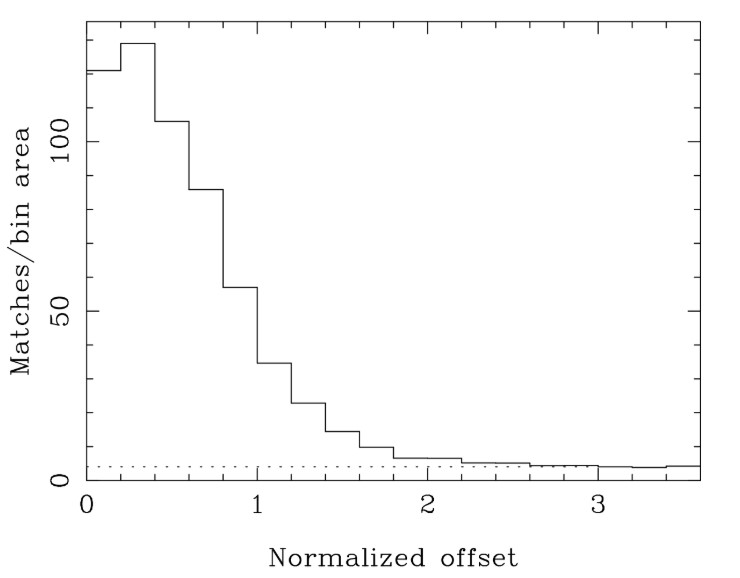
\includegraphics[scale=1]{images/ets_2rxs_match_hist.jpg}}
\caption{The density of ETS-2RXS is plotted as a function normalized offset. The background level is plotted as the horizontal, dotted line. }
\label{imbeded_fb}
\end{figure}

Fig 3.1 displays the number of ETS and 2RXS matches divided by the area of the annulus corresponding to each offset bin as a function of normalized offset.
We can expect the number of 2RXS sources that match to an unrelated ETS source at a given normalized offset away will be proportional to the area of the corresponding bin. Thus, the amount of ETS-2RXS matches that are spurious should be constant as a function of normalized offset.
That amount should then be level in Fig. 3.1.
The excess of match density area above this constant can, therefore, be associated with true matches between the ETS and 2RXS catalog.

\FloatBarrier

In Fig 3.1, the dotted line represents the expected match density due chance coincidences.
The chance coincidence level is computed by averaging the match density values of largest offset bins.
We see that almost no true matches exist beyond a normalized offset of 2.6. The density of chance coincidences allows us to determine the cumulative fraction of true matches as a function of offset (see Table 3.2).
We use this information as a diagnostic for determining a threshold for the normalized offset such that it will yield a sample of highly reliable ETS-2RXS matches.


\begin{table}[H]
    \centering
    \scalebox{0.65}{
    \begin{tabular}{cccccc}
    \hline
    \hline
         bin & number of matches &  number density &  true matches fraction & true number density   & total true matches fraction \\
         \hline
          1  & 121. &  121. &  0.967 &   117. &   0.967 \\
          2   &387. &  129. &  0.969 &  374.9  & 0.968\\
          3 &  530. &  106. &  0.962 &  509.8  & 0.965\\
          4  & 601. &   85.86 &  0.953 &  572.7  & 0.961\\
          5 &  513. &   57.00 &  0.929 &  476.7  & 0.953\\
          6  & 381. &   34.64 &  0.883 &  336.6  & 0.943\\
          7  &297.  &  22.85  & 0.823  & 244.5   &  0.930\\
          8 &  217. &   14.47 &  0.721 &  156.5  & 0.915\\
          9 &  167. &    9.82 &  0.589 &   98.4  &  0.898\\
         10  & 125.  &   6.58 &  0.386 &   48.3  &   0.879 \\        

    \hline
    \hline
    \end{tabular}
    }
    \caption{Breakdown of the match statistics from Fig 3.1 by bin.}
    \label{tab:my_label}
\end{table}

We have adopted a normalized offset cutoff of 1.4.
This yields a sample for which there is a 93\% probability the matches are genuine (only 7\% will be expected spurious matches). 
This results in a catalog of 2,824 match pairs.

After a normalized offset value of 2.6, all matches are likely to be spurious. 
For any ETS that did not match with a 2RXS source with a normal offset value of less than 2.6, the ETS source is considered a not detected in the 2RXS catalog. 
Undetected ETS sources in the 2RXS catalog are expected because of the shallower RASS exposures obtained for most of the sky.
We find that 5,210 ETS sources do not have a counterpart in the 2RXS catalog.



\section{Finding ETS-2RXS Matches in the CSC.2.0}


Now that we have identified a catalog of ETS sources that were also detecteed in the 2RXS, we can further check if they were observed in the CSC2.0. 
The cross matching, in this case, is done differently than that of the ETS and 2RXS cross matching. 
This is due to the way in which the CSC2.0 is accessed and queried.

In order to access the CSC2.0 and all its data products, we use the Chandra Viewer (CSCview).
CSCView is a graphical user interface (GUI) application developed by the Chandra X-ray Observatory that allows access to the CSC2.0 (and all other CSC releases) using user-specified queries. 
Users have the ability to choose per observation properties, stack properties, and master source properties.
To query the CSC2.0, CSCview allows users to input coordinates of one or more sources.
The crossmatch query allows users to input files containing a large number of sources.


\subsection{Initial Search}

We input our catalog of ETS sources that matched to 2RXS sources into CSCview’s cross-match function using the coordinated of the 2RXS sources, as their position errors are typically smaller than those for ETS sources.
The maximum separation allowed between a CSC2.0 source and a source in our catalog to be considered a match is a dynamic value that changes for each source. 
We use the 2.5$\sigma$ 2RXS position uncertainty as the maximum separation allowed. 
With an average 1$\sigma$ 2RXS position error of 12", the average separation allowed is 30".
Under this procedure, the CSCView's cross-matching function outputs a file with the data for all CSC2.0 sources that matched to a source from our input catalog.
Due to the different telescope optics, our results are complex. 
That is, there were 298 ETS-2RXS sources that matched to 853 CSC2.0 sources. 
This result means that there must be some ETS-2RXS sources that have more than one CSC2.0 counterpart.
Therefore, in our analysis of the source matches, we consider single and multiple CSC2.0 matches seperately.

\subsection{ETS-2RXS Sources that Match One CSC2.0 Source}

From the original results that were obtained with the CSCview, we filter to get all uniquely matched ETS-2RXS sources. That is, those for which there is a one-to-one correspondence between the ETS-2RXS catalog source and a CSC2.0 source. 
Of the 298 ETS-2RXS sources, 198 of them have only one CSC2.0 source within the 2.5$\sigma$ 2RXS position error circle. We refer to this list as the single matches list.


\subsection{ETS-2RXS Sources that Match to More than One CSC2.0 Source}

We use the original results that were given by the CSC2.0 again, but this time we are filtering to find all ETS-2RXS that were not uniquely matched. 
This means that there were more than one CSC2.0 source inside the 2.5$\sigma$ position error circle of the 2RXS source.
From the 298 ETS-2RXS sources that had CSC2.0 counterparts, 100 of them had more than one CSC2.0 that they were matched to.
Specifically, there are 100 ETS-2RXS sources that matched 655 CSC2.0 sources.
We refer to this subset of sources as the multiple matches list.

\subsection{Checking for ETS Source Ambiguity}

Using the single matches and the multiple matches lists, we go back to the CSCview. 
This time, rather than using the 2RXS coordinates and position errors, the ETS source positions and position errors are used. 
Similar to what was done in the first iteration where we the coordinates of 2RXS sources, we plug in the ETS-2RXS sources to CSCview.
Because of the poorer spatial resolution of sources in the ETS, false positives are much more likely.
Therefore, stricter criteria for what is considered a match are imposed. 

To ensure that the CSC2.0 sources that already matched an ETS-2RXS (using 2RXS position and position errors) source are being kept, the maximum separation radius is defined slightly differently. 
First, the angular separation between the CSC2.0 source that was already matched to using 2RXS data and the corresponding ETS source are calculated. 
Refer to this value as $\theta$.
The maximum separation searched for CSC counterparts is the 1$\sigma$ ETS position error or $\theta$, whichever is larger.
For the multiple matches, the largest $\theta$ value from all the CSC2.0 match correspdoing to one ETS source or that ETS's  1$\sigma$ position error is used.
Again, the largest of the two is used.
The ETS 1$\sigma$ ETS position error circle values range from 30’’ to 73’’, with an average of 47’.

\subsection{Using the Single Matches List}

We use the single matches list to find CSC2.0 counterparts using the procedure described above. 
Of the 198 sources from the single matches lists, 159 of them also produced a single match when using the ETS coordinates and position error. 
This means that the CSC2.0 source that matched the ETS-2RXS source using the 2RXS positions is the only Chandra source to match an ETS source.
In this case, we have a one-to-one-to-one match.
Figure 3.2 shows this scenario where the CSC2.0 source is within the 2.5$\sigma$ 2RXS position error and within the 1$\sigma$ ETS position error.


\begin{figure}[H]
\centering
\scalebox{0.6}{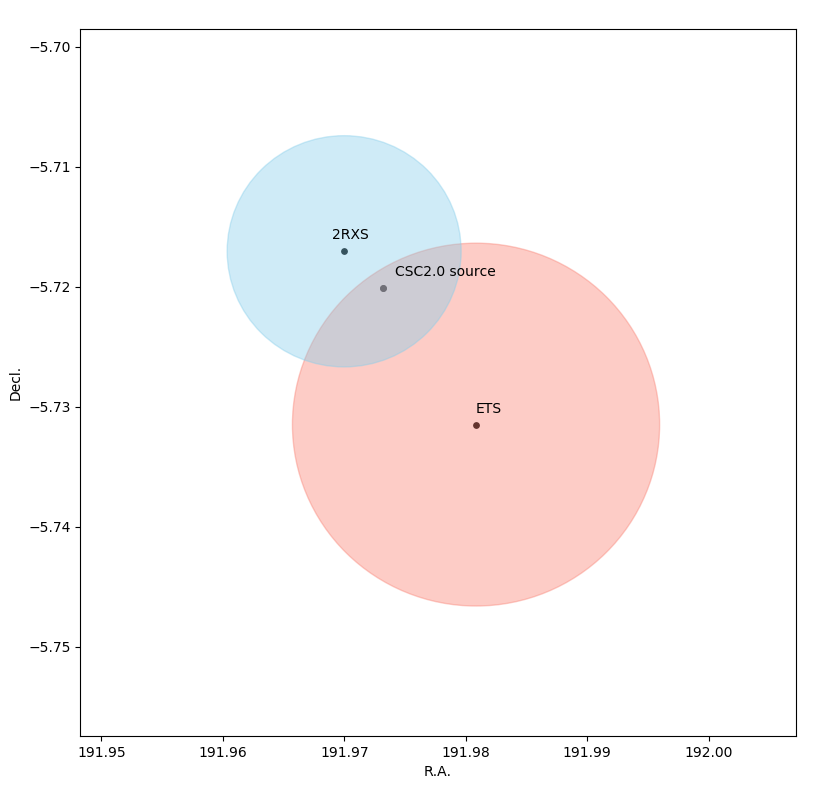
\includegraphics[scale=1]{images/ets_rass_error_circle_w_csc_source.png}}
\caption{The CSC2.0 source found in the intersection of the ETS source's position error circle and the 2RXS source's position error circle. This makes the CSC2.0 source the likely counterpart to both of these sources. }
\label{imbeded_fb}
\end{figure}

For the remainder of the single matches more than one CSC2.0 source is found within the 1$\sigma$ ETS position error. 
Specifically, 39 ETS-2RXS sources match to two or more CSC2.0 sources.
Of those 39, 25 ETS-2RXS had only 2 total CSC2.0 counterparts; 14 has more than 2.
In this case, this field of view for these sources looked similar to that of Fig. 3.3, where there is only one CSC2.0 source in the 2RXS position error circle, but there is at least one more in the ETS position error circle.

\FloatBarrier

\begin{figure}[H]
\centering
\scalebox{0.6}{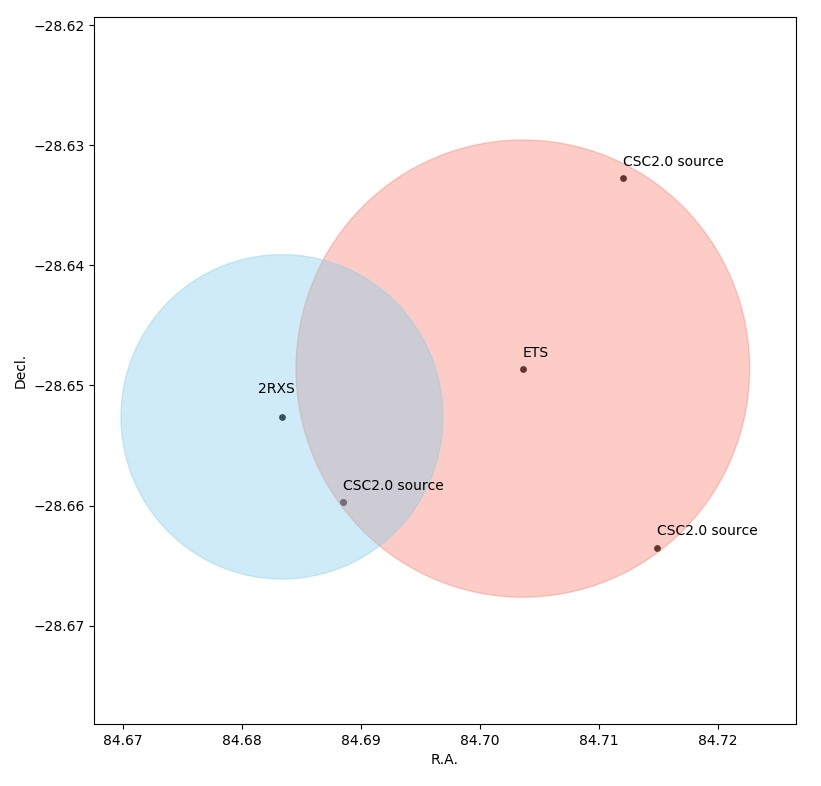
\includegraphics[scale=1]{images/single_rass_multi_ets.jpg}}
\caption{A single CSC2.0 source is found within the 2RXS position error circle but multiple CSC2.0 source are within the ETS position error circle. }
\end{figure}


\FloatBarrier

\subsection{Using the multiple matches list}

Now, we want to take a similar procedure for the multiple match lists as we did for the single match list. 
For each RASS source that matched more than one CSC2.0 sources, we now used the 1$\sigma$ ETS position errors to find CSC2.0 counterparts. 
To define our maximum separation radius, we once again define a  $\theta$ value. 
Theta is the angular separation between the ETS position and the  position of the CSC2.0 source that matched the 2RXS counterpart. 
Because multiple sources match to each of the 2RXS sources in this list, we define a $\theta_{ \text{max}  }$. 
 $\theta_{ \text{max}  }$ is the maximum theta value for any set of CSC2.0 sources corresponding to one ETS-2RXS source. 
Thus, our maximum separation value is the bigger of the following: the  $\theta_{ \text{max}  }$ value or the ETS 1$\sigma$ position error. 
Our original multiple matches list has 100 ETS-2RXS sources that matched two or more CSC2.0 sources. 
Using the ETS coordinates and the procedure just described, we find that some of those 100 ETS-2RXS sources have an additional CSC source within the ETS error circle.
Fig 3.4 shows both the 2RXS position error circle and the ETS position error circle containing multiple CSC2.0 sources.

\begin{figure}[H]
\centering
\scalebox{0.6}{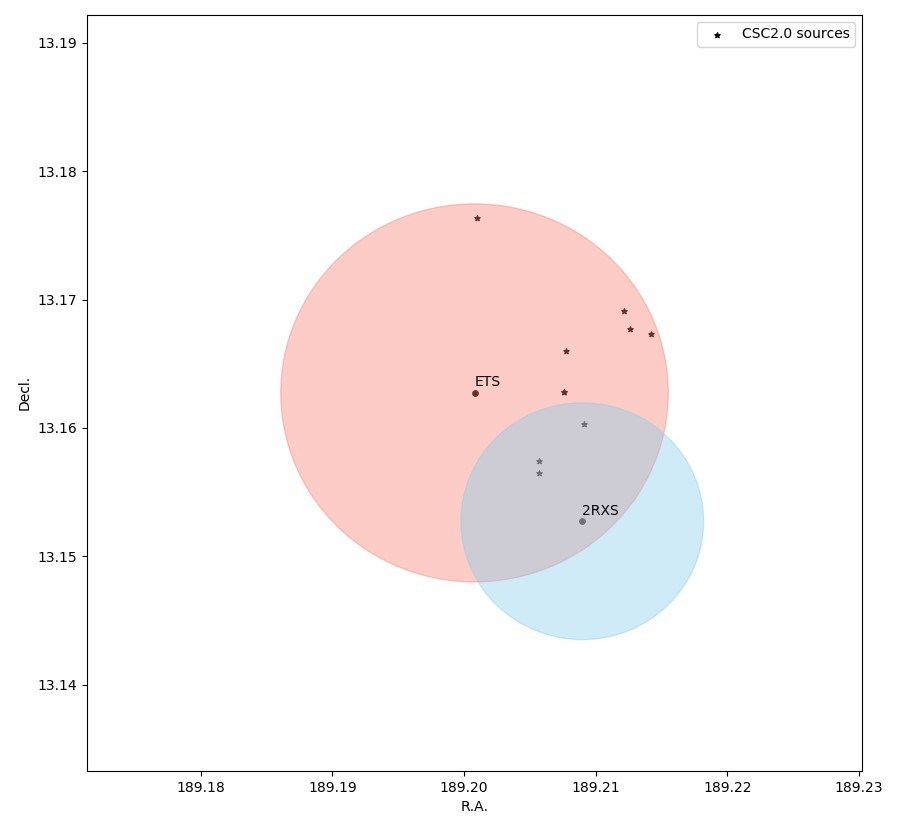
\includegraphics[scale=1]{images/multiple_multiple_pos_err.jpg}}
\caption{Multiple CSC2.0 sources found in the position error circles of the ETS source and the 2RXS source. }
\label{imbeded_fb}
\end{figure}

\subsection{Finding CSC Counterparts for ETS sources not in the 2RXS}

Of the entire ETS catalog, 5,210 of the sources with an SNR ratio above 3.0 did not have a counterpart in the 2RXS catalog. 
These sources, however, can still offer a lot of insight, so we follow a similar procedure for matching them with CSC2.0 sources to identify unambiguous matches between the ETS and CSC2.0 sources. 
Since we don’t have 2RXS to guide our identification of the CSC2.0 counterparts, the way sources are considered matches is a lot stricter. 
That is, only CSC2.0 sources that are within the 1$\sigma$ ETS position error are considered.
To remove any further ambiguity, we consider only matches that are one-to-one.
As ETS position errors can be large, the possibility that many CSC2.0 sources to lie within the position error of one ETS source is significant.
Sticking with the 1$\sigma$ position error circle allows us to be confident that the matches are real and while it is likely some real matches exist outside this radius, the probability of finding multiple CSC2.0 sources increases.
Following this procedudre, of the 5,210 sources, 202 of them matched one-to-one with a source from CSC2.0.




\section{Calculating Source Fluxes}

\subsection{ETS Fluxes}

The fluxes for the ETS sources were computed from their count rates. 
This started by obtaining the response calibration file for Einstein’s IPC instrument from the HEASARC database from NASA/GSFC. 
The response file is made up of components like the effective area curve and the detector redistribution matrix. 
An absorbed power law spectral model is assumed where the power law photon index is taken to be $\Gamma$ = 2.0 and the absorption is set equal to the galactic neutral hydrogen column density ($\text{N}_{ \text{H,gal}  }$) in the direction of a given source. 
The $\text{N}_{ \text{H,gal}  }$ values ranged from 4$\times 10^{19}$ to 3.5$\times 10^{21}$ atoms/cm$^2$.

The response calibration file and the absorbed power-law model are entered in NASA’s XSPEC, a spectral fitting software for X-ray data. 
The energy channel is restricted to the range in which Einstein’s IPC operated: 0.16-3.5 keV and a $\text{N}_{ \text{H,gal}  }$ value is selected from the above range. 
The power-law model is normalized so that XSPEC outputs the estimated count rate of 1.0 counts per second in the 0.16-3.5 keV band. XSPEC then calculates the flux based on this model in the 0.5-2.0 keV band. 

The above process is repeated for 33 different $\text{N}_{ \text{H,gal}  }$ values, all which lie in the range specified. 
With this data, a plot of 0.5-2.0 keV fluxes for 1.0 counts per second vs log($\text{N}_{ \text{H,gal}  }$) is constructed and fitted with a 5th order polynomial.
The polynomial allows us to use the measured $\text{N}_{ \text{H,gal}  }$ value of a source in the ETS catalog, and compute its 0.5-2.0 keV flux for 1 count per second. 
Multiplying by the actual count rate gives the 0.5-2.0 keV flux for the source. 
This is done for all sources in the ETS.


\subsection{2RXS Fluxes}

An almost identical approach is taken to find the fluxes of the 2RXS sources. 
The differences are due to the different properties in ROSAT’s PSPC-C instrument (which is the one that was used for the ROSAT All Sky Survey). 
Specifically, the response calibration files, of course, are different and the energy channel is restricted to an energy band of 0.1-2.4keV.
This results in a 6th order polynomial which is used to compute the 0.5-2.0 keV fluxes of the 2RXS sources.


\subsection{CSC2.0 Fluxes}

Fluxes for the sources in the CSC2.0 are calculated by the Chandra X-ray Center themselves and included as part of the data products available to query. 
The fluxes are calculated in various ways and a user can select the fluxes that best fit their needs.
The fluxes are separated in two main categories based on calculation method: aperture photometry fluxes and spectral model fluxes.

The aperture photometry fluxes are calculated for the master sources and are also calculated for all individual observations. 
For each of these sources, a “best estimate” photon and energy flux is calculated in the 0.5-7.0 keV range. 
Additionally, using the aperture source counts, an aperture model energy flux is also calculated that estimates the power law, blackbody, and bremsstrahlung model flux.

Along with aperture photometry, fluxes are calculated using spectral model fitting. 
This is done for any master source that has a high number of counts ($>$150) in the 0.5 - 7.0 keV range. 
Spectral fits are carried out for a power law model, a blackbody model, and a bremsstrahlung model. 
Each model takes different free parameters to obtain a proper fit. 
The power law model’s free parameters are the neutral hydrogen absorption column density, the power law photon index, and the power law amplitude.
The blackbody model’s free parameters are the neutral hydrogen absorption column density, the blackbody temperature, and the blackbody model amplitude. 
Lastly, the bremsstrahlung model takes the neutral hydrogen absorption column density, the bremsstrahlung temperature, and the bremsstrahlung model amplitude. 
For all the different types of ways in which the fluxes are calculated, the fluxes are reported in the broad (0.5 - 7.0 keV), ultrasoft (0.2 - 0.5 keV), soft (0.5 - 1.2 keV), medium (1.2-2.0 keV), and hard ( 2.0 - 7.0 keV) energy bands \citep{Evans2020}.

Because of how the ETS and 2RXS source fluxes are calculated and in order to have comparable fluxes, we use the aperture photometry power law model fluxes in the 0.5 - 2.0 keV (soft plus medium) energy band.


\section{Flux Ratios of Matched Sources}


With all sources in the catalogs having flux calculations, it is possible to compare the fluxes from the matched pairs that were created from the cross-matching procedure. 
Specifically, flux ratios are calculated to compare the magnitude of the change in flux between the different observations of the same source. 
The flux ratio calculation, however, is different for the singly matched sources and the match pairs with multiple CSC2.0 sources. 
Sources that display a flux ratio of more than a factor of 7 (similar to the source from the \cite{LaMassa2015} paper)  are of particular interest and are considered highly variable. 
At the end of this procedure, we generate a list of X-ray sources that appear to have undergone dramatic variability in their X-ray flux.


\subsection{Flux Ratio for Single Matches}

The flux ratio calculation of singly matched sources is the most straightforward since a direct comparison between the ETS source flux, the 2RXS source flux, and the CSC2.0 source flux can be made. 
The flux ratios are computed between the ETS and 2RXS source, the ETS and the CSC2.0 source, and the 2RXS and CSC2.0 source. 
If any of these ratios are greater than a factor of 7, we consider the source highly variable. 
From the 159 sources in the single-single matches list, 31 of the sources may be highly variable.



\subsection{Flux Ratio for Multiple Matches}

The ETS and 2RXS sources match anywhere from 2 to 10 or more CSC2.0 sources.
After a deep investigation into the matches, it becomes clear that dealing with sources that match to more than 2 CSC2.0 becomes nearly impossible.
Specifically, it is not feasible to determine how a combination of numerous CSC2.0 sources contribute to the observed ETS and 2RXS fluxes.
Thus, it is not possible to assess for X-ray variability in these cases, let alone distinguishing the source of any such variability.

However, we can and do adopt a procedure for carefully handling ETS and 2RXS sources that match to only two CSC2.0 sources.
We only consider match pairs in which (1) the 2RXS source matches two CSC2.0 counterparts within its 2.5$\sigma$ position error circle and the ETS source has no additional CSC2.0 counterparts in its own 1$\sigma$ position uncertainty circle, or (2) the 2RXS source matches to one CSC2.0 source and the ETS counterpart matches only one additional CSC2.0 counterpart.

For match pairs that correspond to first requirement, we can assume that the ETS and 2RXS observations included the flux of both of the CSC2.0 counterparts. 
To untangle the CSC2.0 sources in the ETS and 2RXS observation, consider first the flux for only one of the CSC2.0 sources. 
Let the flux of this CSC2.0 source be labeled C1 and the other flux of the other CSC2.0 source be labeled C2.
Assuming that any change in flux is entirely due to C1, we subtract off C2 from the ETS and 2RXS source fluxes.
This will yield ETS and 2RXS flux values for the CSC2.0 source that can be compared directly to the flux of C1.
Thus, we can compute flux ratios as if it were a single source.
That is, we divide the C2 subtracted ETS and 2RXS fluxes by C1 and assess for variability of the CSC2.0 source corresponding to the C1 flux value.
We can follow an identical procedure for the other CSC2.0 source to compute its flux ratios.
If any of the flux ratios is greater than a factor of 7 (or less than 1/7), we consider the source to be a candidate for high variability.
Our assumption that the change in the flux is entirely due to only one source does not allow us to consider any these sources as more than just candidates.
Following this procedure, we identify 24 match pairs that appear to be highly variable.

For match pairs that meet the second requirement, we assume that the 2RXS flux is composed of only the flux associated with the CSC2.0 source that it matched. 
Let the flux of this CSC2.0 source be labeled C1.
We also assume that the ETS flux is composed of C1 as well as the flux corresponding to the CSC2.0 source that the ETS source matched.
Let the flux for that source be denoted by C2.
Consider first the CSC2.0 source found within the 2RXS position uncertainty circle.
We can divide the 2RXS source flux and the C2 subtracted ETS source flux by C1 assess for variability.
Now consider the CSC2.0 source that is found in the ETS position error circle.
We divide the the C1 subtracted ETS flux by C2 to determine the magnitude of the flux variability.
Again, if any flux ratio is greater than a factor of 7 (or less than 1/7), we consider the source to be a candidate for high variability.
This procedure yields 22 match pairs that appear to be highly variable.

\subsection{Flux Ratio for ETS Sources Not Detected in 2RXS}

The ETS sources that were not detected in the 2RXS but have a CSC2.0 counterpart are also straightforward to compute flux ratios since we only consider the singly matched sources. 
Thus, we can compute the flux ratio between the ETS source flux and the CSC2.0 source flux. 
Among the 202 ETS sources that matched one-to-one with a CSC2.0 source, 46 of them appear to display high variability in the X-ray flux.

For all the matches that appear to have undergone dramatic variability in their X-ray flux, an investigation of their optical properties, including images and spectra, are needed to confirm whether the variability is genuine rather than an artifact related to the differing telescope instrumentation. 


